% This is "sig-alternate.tex" V2.1 April 2013
% This file should be compiled with V2.5 of "sig-alternate.cls" May 2012
%
% This example file demonstrates the use of the 'sig-alternate.cls'
% V2.5 LaTeX2e document class file. It is for those submitting
% articles to ACM Conference Proceedings WHO DO NOT WISH TO
% STRICTLY ADHERE TO THE SIGS (PUBS-BOARD-ENDORSED) STYLE.
% The 'sig-alternate.cls' file will produce a similar-looking,
% albeit, 'tighter' paper resulting in, invariably, fewer pages.
%
% ----------------------------------------------------------------------------------------------------------------
% This .tex file (and associated .cls V2.5) produces:
%       1) The Permission Statement
%       2) The Conference (location) Info information
%       3) The Copyright Line with ACM data
%       4) NO page numbers
%
% as against the acm_proc_article-sp.cls file which
% DOES NOT produce 1) thru' 3) above.
%
% Using 'sig-alternate.cls' you have control, however, from within
% the source .tex file, over both the CopyrightYear
% (defaulted to 200X) and the ACM Copyright Data
% (defaulted to X-XXXXX-XX-X/XX/XX).
% e.g.
% \CopyrightYear{2007} will cause 2007 to appear in the copyright line.
% \crdata{0-12345-67-8/90/12} will cause 0-12345-67-8/90/12 to appear in the copyright line.
%
% ---------------------------------------------------------------------------------------------------------------
% This .tex source is an example which *does* use
% the .bib file (from which the .bbl file % is produced).
% REMEMBER HOWEVER: After having produced the .bbl file,
% and prior to final submission, you *NEED* to 'insert'
% your .bbl file into your source .tex file so as to provide
% ONE 'self-contained' source file.
%
% ================= IF YOU HAVE QUESTIONS =======================
% Questions regarding the SIGS styles, SIGS policies and
% procedures, Conferences etc. should be sent to
% Adrienne Griscti (griscti@acm.org)
%
% Technical questions _only_ to
% Gerald Murray (murray@hq.acm.org)
% ===============================================================
%
% For tracking purposes - this is V2.0 - May 2012

\documentclass[10pt]{main}
\pagenumbering{arabic}

\usepackage{lmodern}
\usepackage[T1]{fontenc}

\usepackage{tabularx, booktabs, array, dcolumn}
\usepackage{dsfont}
\usepackage{listings}
\usepackage{caption}
\usepackage{xcolor}

\newcolumntype{Z}{>{\raggedright}X}

\definecolor{commentsColor}{rgb}{0.497495, 0.497587, 0.497464}
\definecolor{keywordsColor}{rgb}{0.000000, 0.000000, 0.635294}
\definecolor{stringColor}{rgb}{0.558215, 0.000000, 0.135316}

\lstset{
language=C++,
basicstyle=\fontsize{9pt}{10pt}\ttfamily,
numbers=left,
numbersep=5pt,
xleftmargin=14pt,
keepspaces=true,
frame=tb,
framexleftmargin=14pt,
breaklines=true,                 % sets automatic line breaking
captionpos=b,                    % sets the caption-position to bottom
commentstyle=\color{commentsColor}\textit,    % comment style
escapeinside={\%*}{*)},     % if you want to add LaTeX within your code
numberstyle=\tiny\color{commentsColor},
columns=flexible,
showtabs=false,
stringstyle=\color{stringColor},
tabsize=2,
keywords={for, parallel, update, split, rfactor, compute_root, where, compute_at, vectorize},
keywordstyle=\color{keywordsColor}\bfseries,
}

\newcommand{\code}[1]{\texttt{#1}}

\newdef{definition}{Definition}

\newcolumntype{d}{D{.}{.}{2.3}}
\newcolumntype{C}{>{\centering}p}

\begin{document}

% Copyright
%\setcopyright{acmcopyright}
%\setcopyright{acmlicensed}
%\setcopyright{rightsretained}
%\setcopyright{usgov}
%\setcopyright{usgovmixed}
%\setcopyright{cagov}
%\setcopyright{cagovmixed}


\title{Parallel Associative Reductions in Halide}

%\numberofauthors{3}
%\author{
%% 1st. author
%\alignauthor
%Ben Trovato\titlenote{Dr.~Trovato insisted his name be first.}\\
%       \affaddr{Institute for Clarity in Documentation}\\
%       \affaddr{1932 Wallamaloo Lane}\\
%       \affaddr{Wallamaloo, New Zealand}\\
%       \email{trovato@corporation.com}
%% 2nd. author
%\alignauthor
%G.K.M. Tobin\titlenote{The secretary disavows
%any knowledge of this author's actions.}\\
%       \affaddr{Institute for Clarity in Documentation}\\
%       \affaddr{P.O. Box 1212}\\
%       \affaddr{Dublin, Ohio 43017-6221}\\
%       \email{webmaster@marysville-ohio.com}
%% 3rd. author
%\alignauthor Lars Th{\o}rv{\"a}ld\titlenote{This author is the
%one who did all the really hard work.}\\
%       \affaddr{The Th{\o}rv{\"a}ld Group}\\
%       \affaddr{1 Th{\o}rv{\"a}ld Circle}\\
%       \affaddr{Hekla, Iceland}\\
%       \email{larst@affiliation.org}
%}

\maketitle
\begin{abstract}

  Halide is a domain-specific language for fast image processing that separates pipelines into the \emph{algorithm}, which defines \emph{what} values are computed, and the \emph{schedule}, which defines \emph{how} they are computed. Changes to the schedule are guaranteed to not change the results. While Halide supports parallelizing and vectorizing naturally data-parallel operations, it does not support the same scheduling for reductions. Instead, the programmer must create data parallelism by manually factoring reductions into multiple stages. This manipulation of the \emph{algorithm} can introduce bugs, impairs readability and portability, and makes it impossible for automatic scheduling methods to parallelize reductions.

  We describe a new Halide scheduling primitive \code{rfactor} which moves this factoring transformation into the \emph{schedule}, as well as a novel synthesis-based technique that takes serial Halide reductions and synthesizes an equivalent binary associative reduction operator and its identity. This enables us to automatically replace the original pipeline stage with a pair of stages which first compute partial results over slices of the reduction domain, and then combine them. Our technique permits parallelization and vectorization of Halide algorithms which previously required manipulating both the algorithm and schedule.

\end{abstract}


%
%  Use this command to print the description
%
\printccsdesc

%\keywords{ACM proceedings; \LaTeX; text tagging}

\section{Introduction}
\label{introduction}
Halide \cite{Ragan-Kelley:2013:HLC:2491956.2462176} is a domain-specific language designed for fast image processing and computational photography. Halide decouples the \emph{algorithm}, which defines \emph{what} values are computed, from the \emph{schedule}, which defines \emph{how} values are computed. Halide guarantees consistency -- an algorithm produces the same results no matter the schedule. Programmers are thus free to explore the space of schedules without introducing correctness bugs, and can vary the schedule per architecture without producing different results on different platforms.

Data-parallel operations, such as resizing an image, can be easily parallelized or vectorized in Halide. However, Halide does not support the same scheduling manipulations on reductions. To parallelize or vectorize a reduction, the programmer has to manually factor the reduction into multiple stages to expose new data parallelism. For example, instead of computing the histogram of an entire image, one might instead write an algorithm that computes the histogram of each row, and then adds those partial histograms. This need to rewrite the algorithm violates the core tenet of Halide: The algorithm should only specify \emph{what} is computed. It is the role of the schedule to specify \emph{how}. This manipulation of the \emph{algorithm} to parallelize reductions is bug-prone and hampers readability and portability. It is a language wart.

In this work, we present a new Halide scheduling primitive called \code{rfactor}, which moves this factoring of a reduction into the \emph{schedule}, while maintaining Halide's consistency guarantees. \code{rfactor} takes a Halide serial reduction (expressed with an unstructured Halide \emph{update} definition), and synthesizes the equivalent binary associative reduction operator and its identity. In some cases this synthesis problem is trivial. For example, given Halide code that sums a one-dimensional vector (Listing~\ref{lst:sum}), it is straightforward to deduce that the binary operator involved is addition, and its identity is zero. In other cases this synthesis problem is more challenging. Listing~\ref{lst:complex_magnitude} shows Halide code that finds the complex number with the greatest magnitude and its location within a two-dimensional array. It is not obvious what the equivalent associative binary operator is for this algorithm.

During the compilation process, \code{rfactor} splits the original serial reduction into a pair of stages: The \emph{intermediate} stage computes partial results over slices of the domain of the reduction, and the \emph{merge} stage combines those partial results. The intermediate stage is now data parallel over the slices, which means that it can now be vectorized or parallelized using Halide's existing scheduling primitives.

Combined with other Halide scheduling primitives, such as \code{split}, \code{rfactor} allows Halide to represent a broad class of schedules for parallel and vectorized reductions. For example, rfactor can express several divide-and-conquer strategies for parallelizing and vectorizing the summation of a one-dimensional array (see Figure \ref{fig:rfactor}).

\begin{figure}
\centering
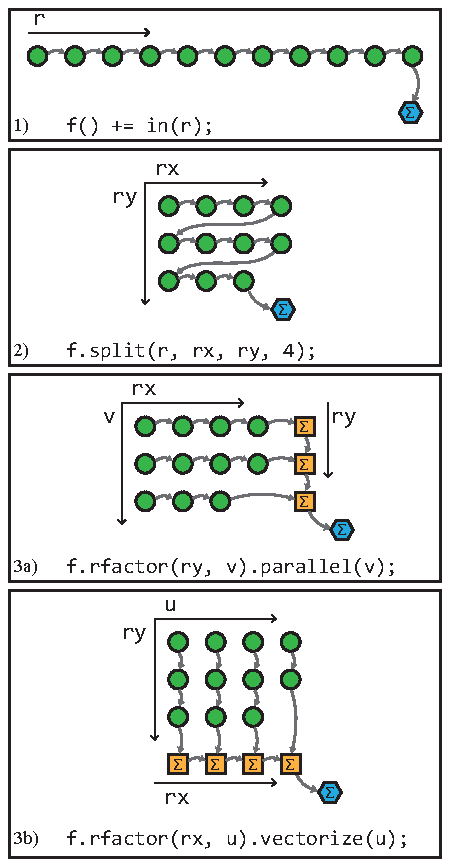
\includegraphics[width=3.2in]{rfactor}
\caption{
\code{split} followed by \code{rfactor} used to vectorize or parallelize a one-dimensional summation. 1) A serial summation of 11 elements over a one-dimensional domain \code{r}. 2) The \code{split} scheduling directive reshapes the domain into a two-dimensional reduction. The reduction is still serial. 3a) The \code{rfactor} directive creates and returns a new (orange) \emph{intermediate} stage which computes partial results along each row. The intermediate stage is now data parallel over its outer loop, which is now indexed with the new pure variable \code{v}. The merge stage (blue) retains only the serial loop over the reduction variable \code{ry}. We have \emph{reassociated} the summation. 3b) Alternatively, one can use rfactor to make the \emph{inner} loop data parallel. This can be used to vectorize reductions. The intermediate stage computes sums of whole vectors, data parallel across the vector lanes, and then the merge stage sums the lanes of the vector result. The strategy in 3a and 3b can be combined to both vectorize \emph{and} parallelize a summation.
}
\label{fig:rfactor}
\end{figure}

\code{rfactor} further separates the \emph{algorithm} from its \emph{schedule} by making it possible to factor reductions using the schedule alone. In addition to the readability and portability benefits, this means that tools that automatically generate schedules (\cite{Mullapudi:2016:ASH:2897824.2925952},\cite{Ragan-Kelley:2013:HLC:2491956.2462176}) are now capable of parallelizing reductions, which was previously a task outside of their purview.

Our work makes the following contributions:
\begin{itemize}
  \item We introduce a new Halide scheduling primitive \code{rfactor} which factors a Halide reduction into pair of reductions: an \emph{intermediate} stage that computes partial results over slices of reduction domain and \emph{merge} stage that combines those partial results;
  \item We descibe a method for automatic synthesis of an equivalent associative binary reduction operator and its identity from a serial reduction expressed as an imperative Halide \emph{update}.
  \item We implement a new stage in the Halide compiler that matches arbitrary reductions with a set of XXX fragments that are pre-generated using our synthesis method, and show that this enables the compiler to effectively transform a large set of reductions into their parallel equivalents.
\end{itemize}

The paper is structured as follows. Section~\ref{background} provides background on Halide and a discussion of related work. Section~\ref{assoc_red} presents the \code{rfactor} scheduling primitive and how it transforms Halide programs. Section~\ref{synthesize} describes the associative binary reduction operator synthesis technique. Section~\ref{evaluation} describes limitations of the technique, and demonstrates that this technique does indeed produce the expected performance gains from vectorization and parallelization.

\begin{lstlisting}[
caption = {Halide sum reduction over a one-dimensional vector.}, label={lst:sum}]
Func out;
out() = 0;
RDom r(0, input.width());
out() = out() + input(r.x);
\end{lstlisting}

\begin{lstlisting}[
caption = {Halide reduction which finds the complex number with the greatest magnitude and its location in a two-dimensional array.}, label={lst:complex_magnitude}]
Func out;
out() = {0, 0, 0, 0};
RDom r(0, input.width(), 0, input.height());
Expr real = input(r.x, r.y)[0];
Expr imag = input(r.x, r.y)[1];
Expr mag = real * real + imag * imag;
Expr best_mag = out()[0] * out()[0] +
                out()[1] * out()[1];
Expr c = mag > best_mag;
out() = {select(c, real, out()[0]),
         select(c, imag, out()[1]),
         select(c, r.x, out()[2]),
         select(c, r.y, out()[3])};
\end{lstlisting}


\section{Background and Related Work}
\label{background}
Programmer defines \emph{algorithm} in Halide through a Halide \emph{function}. Halide \emph{function} consists of sequence of stages, and is the unit by which we schedule things. By default, each of these stages represents a perfectly-nested loop nests in which a single value of the \emph{function} is computed and stored in the innermost loop per iteration. Stages beyond the first are called \emph{update} stages, and are allowed to recursively refer to the function. Some of the loops are data parallel and are constrained to be race-condition free by syntactic restrictions. These are represented as \code{Var}s. The bounds of these loops are inferred by Halide using interval arithmetic. Some other loops may have user-specified bounds and a user-specified nesting order, and fewer syntactic restrictions on their use. These are known as \code{RVar}s, which comprise \code{RDom}s. \code{RVar}s are used to express reductions, scattering, scans, etc. Each of these loop types, \code{Var} and \code{RVar}, can be manipulated in various ways through Halide scheduling primitives: they can be tiled, unrolled, mutually interchanged, etc., provided that the nesting order of \code{RVar}s is respected. 

While \code{Var}s are safe to parallelize or vectorize by construction -- \code{Var}s represents the naturally data-parallel axes of an \emph{algorithm} -- , \code{RVar}s can be parallelized or vectorized if and only if Halide can prove that no race condition exists. This makes parallelizing or vectorizing stages that use only \code{RVar}s difficult. For example, consider the two-dimensional convolution blur kernel shown in Listing \ref{lst:blur_loopness}, which is easily parallelizable across \code{Var} $x$ and $y$. Histogram of an image (see Listing \ref{lst:histogram_loopness}), on the other hand, is harder to parallelize since its update stage only involves \code{RVar}s. In order to parallelize a reduction like histogram, one needs to be able to factorize it into slices that have no dependencies on each other.

Although there have been several works in automatic generation of parallel associative reductions from a serial reduction, most of those works assume an explicit associative binary reduction operator, which is not applicable to Halide. Since Halide does not support reduction using a binary operator as a first-class primitive, reduction in Halide is implemented through usage of non-data-parallel \code{RVar}s. For Halide to support parallel reductions, it needs to be able to deduce an equivalent binary associative reduction operator and its identity from a serial reduction expressed as an imperative Halide \emph{update}. 

Prior work by Morita et al.~\cite{Morita:2007:AIG:1250734.1250752} introduced automatic generations of divide-and-conquer parallel programs framework based on the third homomorphism theorem and derivation of weak-right inverse. However, it requires programmer to specify the leftwards and rightwards forms of the sequential function which may not be obvious to derive. Teo et al.~\cite{Teo:1997:DEP:266670.266697} proposed a method to synthesize parallel divide-and-conquer
programs from recurrence function (which has the closest form to Halide serial reduction) through induction. They first derive two equivalent pre-parallel forms of the recurrence function by applying some generalization rules and deduce the "unknowns", the intermediate and merge reduction functions, through induction of those two pre-parallel forms. Although, it can be applied to solve some complex recurrences, such as reduction of complex multiplication, it requires long derivation and is unable to deal with argmin, which requires non-trivial re-ordering of chain of select nodes during the induction steps. 

Superoptimization~\cite{Granlund:1992:EBU:143095.143146, Massalin:1987:SLS:36206.36194} searches for the shortest or most optimized way to compute a branch-free sequence of instructions, by exhaustively searching over a space of possible programs. These rewrites can then be turned into peephole optimizations in compilers. More recent work has used stochastic search~\cite{Phothilimthana:2016:SUS:2872362.2872387, Schkufza:2013:SS:2490301.2451150} and program synthesis~\cite{Lopes:2015:PCP:2737924.2737965} to find replacements for larger sequences of instructions. Smith et al.~\cite{Smith:2016:MPS:2908080.2908102} used program synthesis to automatically generate MapReduce-style distributed programs from input-output examples. 

In this work, we find equivalent replacements of a Halide reduction through a combination of enumeration and synthesis; in addition, though our domain is more restricted, we search for larger replacements than most superoptimizers.


\begin{lstlisting}[caption={Convolution blur kernel is easily parallelizable across \code{Var} $x$ adn $y$}, label={lst:blur_loopness}]
// First stage
for y in range(input.height()):
  for x in range(input.width()):
    blur[x][y] = 0
// Update stage
parallel for y in range(input.height()):
  parallel for x in range(input.width()):
    for ry in range(kernel.height()):
      for rx in range(kernel.width()):    
        blur[x][y] = 
          blur[x][y] + 
          kernel[rx][ry]*input[x+rx-1][y+ry-1] 
\end{lstlisting}

\begin{lstlisting}[caption={Histogram of an image is hard to parallelize since its update stage does not involve \code{RVar}s}, label={lst:histogram_loopness}]
// Serial version
// First stage
for x in range(256):
  hist[x] = 0
// Update stage
for ry in range(input.height()):
  for rx in range(input.width()):
    hist[clamp(int(input[rx][ry]), 0, 255)] += 1
\end{lstlisting}


\section{The \code{rfactor} Transformation}
\label{assoc_red}
\subsection{Reductions in Halide}

Serial reductions in Halide (e.g. summation over an array, histogram, etc.) are implemented using \code{RVar}s or \code{RDom}s. An \code{RVar} is an implicit serial loop, and an \code{RDom} is an ordered list of \code{RVar}s specifying a serial loop nest. Since \code{RVar}s are not trivially parallelizable or vectorizable, a programmer must manually \emph{factor} a reduction into an \emph{intermediate} function that performs reduction over distinct slices of the domain, and a \emph{merge} function that combines those partial results.

This manual manipulation is tedious and error-prone, especially when the reduction domain is non-rectangular (see Listing \ref{lst:circular_max_1}). To further complicate matters, it is hard to infer what binary reduction operator is equivalent to a Halide update definition, and even then, many binary operators are not obviously associative (e.g. $x + y + 7xy$ is in fact associative). We will defer these issues to section \ref{synthesize}, and for now assume that given a Halide update definition we can deduce the equivalent associative binary operator and its identity. Note that we do not require the binary operators to be commutative.

\subsection{The \code{rfactor} Transformation}

To remove the burden of \emph{factoring} a reduction from the programmer, we introduce a new scheduling primitive called \code{rfactor}. This splits a reduction into pair of reductions, which we will call the \emph{intermediate} stage and the \emph{merge} stage. \code{rfactor} takes as input a list of \code{<RVar, Var>} pairs. \code{RVar}s not in the list are removed from the \emph{merge} stage and lifted to the \emph{intermediate} stage. The remaining \code{RVar}s become \code{Var}s in the \emph{intermediate} stage, which allows them to be parallelized or vectorized. See Figure \ref{fig:rfactor} for a simple example. The listings below demonstrate more complex usage.

 Note that we limit the scope of \code{rfactor} to reductions where the \emph{intermediate} and \emph{merge} stages have the same equivalent binary associative reduction operator. For instance, if the equivalent binary associative reduction operator of the \emph{intermediate} stage is \code{min(x, y)}, then that of the \emph{merge} stage must also be \code{min(x, y)}. Another restriction is that the binary associative operator must have an identity, as it is used to initialize the \emph{intermediate} stage. Not all associative binary operators have identities (e.g. $2xy$, where $x, y \in \mathds{Z}$).

\begin{lstlisting}[caption={Computing the histogram of a two-dimensional image in Halide. The RDom defines an implicit loop nest over \code{r.x} and \code{r.y}. Halide will not permit either of these loops to be parallelized, as that would introduce a race condition on the += operation.}, label={lst:histogram_rfactor_1}]
// Algorithm
Func hist;
Var i;
hist(i) = 0;
RDom r(0, input.width(), 0, input.height());
hist(input(r.x, r.y)) += 1;

// Schedule
hist.compute_root();
\end{lstlisting}

\begin{lstlisting}[caption={A manually-factored histogram. The programmer has introduced an intermediate function that computes the histogram over each row of the input. This intermediate is data-parallel over y, and so it can be parallelized. The original function \code{hist} now merely sums these partial histograms. It is data-parallel over histogram buckets, and the programmer has vectorized it.}, label={lst:histogram_rfactor_2}]
// Algorithm
Func intm;
Var i, y;
intm(i, y) = 0;
RDom rx(0, input.width());
intm(input(rx, y)) += 1;

Func hist;
hist(i) = 0;
RDom ry(0, input.height());
hist(i) += intm(i, ry);

// Schedule
intm.compute_root().update().parallel(y);
hist.compute_root().update().vectorize(i, 4);
\end{lstlisting}

\begin{lstlisting}[caption={Using \code{rfactor}, the programmer can produce the same machine code as in \ref{lst:histogram_rfactor_2}, using the simpler algorithm in \ref{lst:histogram_rfactor_1}. While the schedule is more complex, recall that it is only the five lines of algorithm that determines correctness. The programmer was able to transform the code to exploit parallelism without risking introducing a correctness bug.}, label={lst:histogram_rfactor_3}]
// Algorithm
Func hist;
Var i;
hist(i) = 0;
RDom r(0, input.width(), 0, input.height());
hist(input(r.x, r.y)) += 1;

// Schedule
Var y;
hist.compute_root()
Func intm = hist.update().rfactor(r.y, y);
intm.compute_root().update().parallel(y);
hist.update().vectorize(i, 4);
\end{lstlisting}

\begin{lstlisting}[caption={Computing the maximum over a circular domain. Reduction domains need not be rectangular. In this case we use \code{RDom::where} to restrict it to the points that lie within a circle of radius 10.}, label={lst:circular_max_1}]
// Algorithm
Func max_val;
max_val() = 0;
RDom r(0, input.width(), 0, input.height());
r.where(r.x*r.x + r.y*r.y <= 100);
max_val() = max(max_val(), input(r.x, r.y));

// Schedule
max_val.compute_root();
\end{lstlisting}

\begin{lstlisting}[caption={Manually factoring this reduction requires also manipulating the predicate associated with the RDom. The identity for \code{max} is the minimum value of the type in question.}, label={lst:circular_max_2}]
// Algorithm
Func intm;
Var y;
intm(y) = input.type().min();
RDom rx(0, input.width());
rx.where(rx*rx + y*y <= 100);
intm(y) = max(intm(y), input(rx, y));

Func max_val;
max_val() = 0;
RDom ry(0, input.height());
max_val() = max(max_val(), intm(ry));

// Schedule
intm.compute_root();
    .update().parallel(y);
max_val.compute_root();
\end{lstlisting}

\begin{lstlisting}[caption={Using \code{rfactor} in the schedule can produce the same machine code from the simpler form of the algorithm.}]
// Algorithm
Func max_val;
max_val() = 0;
RDom r(0, input.width(), 0, input.height());
r.where(r.x*r.x + r.y*r.y <= 100);
max_val() = max(max_val(), input(r.x, r.y));

// Schedule
Var y;
max_val.compute_root();
Func intm = max_val.update().rfactor(r.y, y);
intm.compute_root();
    .update().parallel(y);
\end{lstlisting}




\section{Synthesizing Associative Binary Operators}
\label{synthesize}
% Overview of section
In the previous section, we described how \code{rfactor} transforms a Halide reduction to expose new data parallelism. Doing so requires synthesizing the associative binary operator equivalent to the Halide \emph{update} definition being factored. In this section we describe how we do this synthesis.

% Set up problem, LUT solution
In some cases generating the equivalent associative operator from an update definition is trivial (e.g.\ summation). In other cases it is not, especially when the function reduces onto multiple values (see the examples in Figure~\ref{fig:subgraphs}). The \emph{inverse} problem is easier: Given an associative binary operator, it is straightforward to generate the Halide update definition that implements reduction by it. Therefore, if there were a \emph{small} finite set of associative binary operators, we could simply attempt to match the update definition being factored against each of them in turn. Halide already includes facilities for doing regex-like matching of expressions against patterns with wildcards. Unfortunately, there are more meaningful associative binary operators than could reasonably be thought of ahead of time by a compiler author.

% Full synthesis solution
An alternative approach is to use program synthesis techniques~\cite{Solar-Lezama:2008:PSS:1714168, Torlak:2013:GSL:2509578.2509586} to synthesize the corresponding associative reduction at compile-time when the call to \code{rfactor} is made. This is intractably slow, and can increase compile times of Halide pipelines from seconds to hours.

% Our solution
We use a hybrid of the two approaches, amplified with a strategy for decomposing each synthesis problem into several simpler problems. The overall strategy is shown in Figure~\ref{fig:system}.  Offline, we generate a large finite table of one- and two-dimensional \emph{elementary} associative binary operators and their identities. These are akin to primes -- they are the associative operators which cannot be decomposed into a combination of simpler associative binary operators. The table also records whether each operator is commutative. At compile-time, we decompose the given Halide update definition into a composition of simpler, lower-dimensional definitions in the same way, then search the table for the elementary operator corresponding to each. If consistent matches are found, we reassemble the results into a composite associative operator equivalent to the original update definition. In Section~\ref{subsec:generation} we describe how we generate the table, and in Section~\ref{subsec:decomposition} we describe the decomposition procedure.

\begin{figure}[tb]
\centering
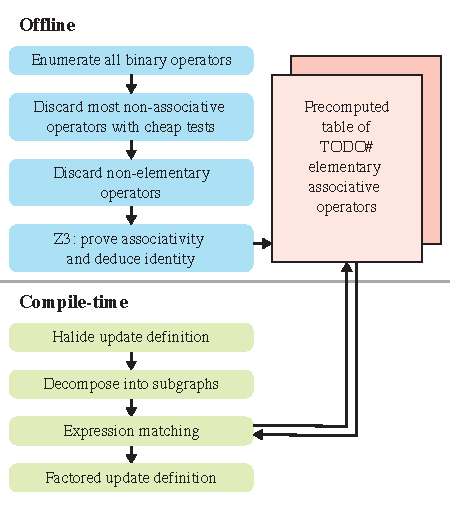
\includegraphics[width=3.2in]{system}
\caption{To factor a reduction written as a Halide update definition, we must first synthesize the equivalent associative binary operator. We generate a large table of elementary associative operators offline by enumerating all non-trivial expression trees and filtering out the ones that are not associative operators. At compile-time, we then decompose the given update definition into simpler definitions and match each against the table. Combining the results gives us the equivalent associative binary operator, which we can use to generate the factored form of the reduction.}
\label{fig:system}
\end{figure}



\subsection{Generating Elementary Operators}
\label{subsec:generation}

We begin with an enumeration of all one- and two-dimensional tuples of expression trees in two tuple inputs $x$ and $y$. The operators used to form the inner nodes of the trees are Halide's IR nodes (\code{*}, \code{+}, \code{-}, \code{min}, \code{max}, \code{select}, \code{<}, etc). We can reject some classes of uninteresting expressions by excluding them from the enumeration altogether.

\begin{enumerate}
\item We only generate trees which use both $x$ and $y$.
\item During matching we canonicalize both the pattern and the input expression using the Halide simplifier and solver; thus, we can make the enumeration more tractable by only generating trees that are already in canonical form.  The canonicalization strategy moves all instances of a variable in an expression tree as far to the left and as far up the tree as possible. We canonicalize expressions to the following form: wherever possible, $x_i$ is to the left of $x_{i+1}$ and any $y_j$ is to the left of $y_{j+1}$. Constants are always on the right.
\item We generate trees using a single generic constant $k$, rather than generating trees containing all possible constants as leaves.
\item We do not generate trees that would be trivially simplified. For example, we do not generate subexpressions like $max(x_0, x_0)$.
\end{enumerate}

After generating a large set of candidate expressions in this manner, we then subject the expressions to a battery of tests so that only elementary associative operators remain. The tests are arranged in increasing order of expense, so that we can cheaply reject most expressions.

\begin{enumerate}
\item For an operator $f$, we construct the expressions $f(f(x, y),$ $z)$ and $f(x, f(y, z))$, and substitute in 100 randomly-selected values for $x, y, z, k$. If the two expressions don't evaluate to the same thing, the expression is not associative and can be rejected.
\item We then reject operators which can be decomposed using the decomposition procedure in Subsection~\ref{subsec:decomposition}.
\item Finally, to \emph{prove} that the expression is associative, we use the Z3~\cite{DeMoura:2008:ZES:1792734.1792766} SMT solver to verify that $\forall x, y, z, k \;\;f(f(x, y), $ $z) = f(x, f(y, z))$, where $k$ is the constant contained within the function $f$. If this proof succeeds, we then ask Z3 to solve $\forall x, k \;f(id, x) = x$ to synthesize the identity $id$ and to decide its commutativity. This commutativity flag is used to determine the validity of calling \code{rfactor} on the inner loop dimensions of an associative reduction.
\end{enumerate}

In the table of expressions that this produces, $x$ represents the partial result being reduced onto, and $y$ is a wildcard which could match any expression. When matching, $x$ must also appear on the left-hand-side of the update definition. $y$ may depend on the reduction domain coordinates, but may not depend on the partial results. The constant $k$, if it exists, may match anything which neither depends on the reduction domain coordinates nor the partial result. For example, the update definition which separately computes the sum-of-squares of the even and odd values of some input \code{in} could be written as:

\code{f(in(r)\&1) = f(in(r)\&1) + in(r)*in(r)}

\noindent This would match against the pattern $x = x + y$, where $x$ matches \code{f(in(r)\&1)}, and $y$ matches \code{in(r)*in(r)}.

We terminate the enumeration at trees with 8 leaves for the purposes of the experiments described in this work. Since some operations are associative in certain scalar types and not others, we generate different tables for each of Halide's scalar types.  This takes 1.5 days and generates around 9,000 elementary operators to match against per type. Many of the operators are simple operators written in a complex way: as we wish to catch all ways in which a programmer might write a reduction, we make no attempt to exclude these from the table. For faster retrieval, the table of each Halide's scalar type is split into subtables based on the root IR node (e.g. \code{Add}, \code{Mul}, etc.) of the expression. Within each subtable, the operators are ordered based on the total number of leaves (simple expressions are located at the top of the table since they are more likely to be encountered in practice). The operators we use are \code{Add}, \code{Sub}, \code{Mul}, \code{Min}, \code{Max}, comparisons, and \code{Select} (Halide’s if-then-else construct). We then linearly scan the sub-table searching for a matching expression. The first 10 elementary associative operators for signed 32-bit integers are shown in Listing~\ref{fig:top10}.

\begin{figure}
\centering
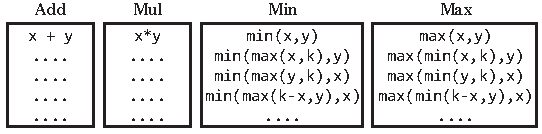
\includegraphics[width=\columnwidth]{tables}
\caption{The first 10 elementary associative operators for 32-bit signed integers organized into subtables based on the root IR node, with simpler expressions located at the top. The boolean flag on the left indicates the commutativity of the expression.}
\label{fig:top10}
\end{figure}

%\begin{lstlisting}[float,caption={The first 10 elementary associative operators for 32-bit signed integers}, label={lst:top10}]
%x + y
%x * y
%min(x, y)
%max(x, y)
%max(min(x, k), y)
%min(max(x, k), y)
%max(min(y, k), x)
%min(max(y, k), x)
%max(min(k - x, y), x)
%min(max(k - x, y), x)
%\end{lstlisting}

%As the list grows, operators become more and more esoteric. An example 8-leaf operator from the list for unsigned integers is TODO

As we only consider one- and two-dimensional expressions, there are meaningful primitive operators that we never discover. For example, we never generate quaternion multiplication, since it is an elementary associative operator in 4 tuple elements, where every expression tree has 8 leaf nodes. We must add any important higher-dimensional primitive operators to our table manually.

%Another limitation is that for each associative reduction, we have a single pattern for the update definition we expect to see, and so if the Halide simplifier and solver fail to canonicalize an update definition into that form, we will not recognize it. For example, consider the reduction which counts how many points in the reduction domain satisfy some predicate $P$. It may be written with the addition outermost:

%\code{f() = select(P(r), 1, 0) + f()}

%After canonicalization we recognize this as a sum reduction of the form \code{x = x + y}. One might also write it with the \code{select} outermost:

%\code{f() = select(P(r), f() + 1, f())},

%We do not recognize this as a sum reduction.

\begin{figure}[tb]
\centering
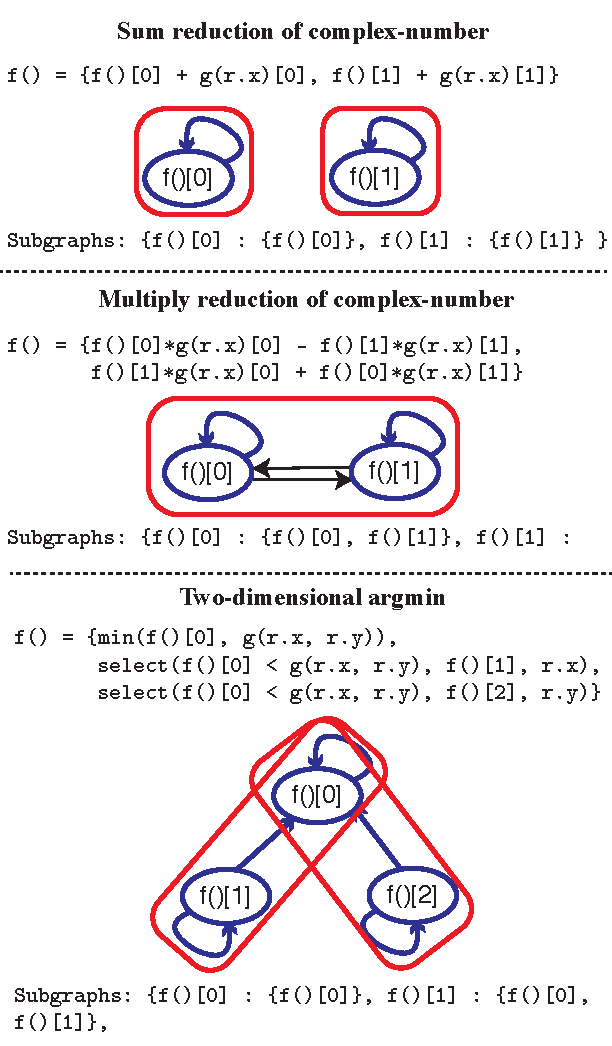
\includegraphics{subgraphs}
\caption{Dependency graphs of various multi-valued Halide \emph{update} definitions. Their subgraph decompositions are shown in red dotted circle. To find the associative operator equivalent to a complex Halide update definition, we first decompose it into subgraphs, then search for each subgraph in our precomputed table of elementary operators, then recompose the results into a single multi-valued associative operator.}
\label{fig:subgraphs}
\end{figure}

\subsection{Subgraph Decomposition}
\label{subsec:decomposition}

To describe how we decompose reductions into elementary operators, we must first discuss how one might \emph{compose} elementary reductions. The simplest way to compose two reductions into a higher-dimensional reduction is to compute them at the same time, independently. This means that reductions that are a concatenation of smaller independent associative reductions are also associative. For example, the tuple computation:

\code{f() = \{f()[0] + in(r), f()[1] * in(r)\}}

is associative, because it is a composition of the following two associative reductions:

\code{f0() = f0() + in(r)}

\code{f1() = f1() * in(r)}

Secondly, if we have an associative operator in which two tuple elements compute the same value, we can deduplicate it, reducing the dimensionality by one. The result is still associative. Therefore, we can prove a reduction is associative by duplicating one of the elements to break a dependency and then applying the rule above. Consider the case of two-dimensional \code{argmin}:

\begin{lstlisting}
f() = {
  min(f()[0], in(r.x, r.y)),
  select(f()[0] < in(r.x, r.y), f()[1], r.x),
  select(f()[0] < in(r.x, r.y), f()[2], r.y)}
\end{lstlisting}

The three tuple elements are the minimum value, and its $x$ and $y$ coordinate. All three tuple elements depend on the minimum value \code{f()[0]}, so we cannot decompose this into independent reductions immediately. Let us duplicate the first tuple element to break the dependency:

\begin{lstlisting}
f() = {
  min(f()[0], in(r.x, r.y)),
  select(f()[0] < in(r.x, r.y), f()[1], r.x),
  min(f()[2], in(r.x, r.y)),
  select(f()[2] < in(r.x, r.y), f()[3], r.y)}
\end{lstlisting}

There are now no dependencies between the first two elements and the last two. This is a simple concatenation of two single-variable \code{argmin} operations. Single-variable \code{argmin} uses two tuple elements, and is present in our table of primitive operators, so we recognize two-dimensional \code{argmin} as associative via its decomposition into two one-dimensional \code{argmin} reductions.

In general we consider the directed graph of dependencies between tuple elements. There is a vertex per tuple element, and an edge from vertex $i$ to vertex $j$ whenever the definition of tuple element $i$ refers to tuple element $j$. If we repeatedly duplicate vertices (tuple elements) to break dependencies, in the limit the graph has one connected component per original tuple element, and that component is the subgraph containing the vertices reachable from that tuple element. If each such subgraph is an associative reduction, then the original reduction is associative. See Figure~\ref{fig:subgraphs} for several examples.

%The general way to apply these two rules to decompose an arbitrary reduction into its components is to construct the directed graph $G$ of dependencies between tuple elements. There is a vertex $N_i$ for each tuple element $i$, and there is an edge from $N_i$ to $N_j$ whenever the value of tuple element $i$ depends on tuple element $j$. The two rules above can then be stated as:

%\begin{enumerate}
%\item If every connected component of $G$ is an associative reduction, then $G$ is an associative reduction.
%\item If we duplicate one of the nodes of $G$, partitioning its incoming edges arbitrarily between the two copies, then the resulting graph is associative iff $G$ is associative, as they compute the same thing.
%\end{enumerate}

% This is a shitty ``proof''
%Let the subgraph $S_i$ be all vertices and edges reachable from $N_i$. We can make a copy of $S_i$ as its own connnected component set apart from the rest of $G$ by the following procedure: Initialize $S_i$ to contain only a duplicate of $N_i$, with no incoming edges. Then repeatedly consider all edges that leave $S_i$, and make duplicates of the vertices they point to, where edges from vertices within $S_i$ point to the duplicate, and edges from vertices not in $S_i$ point to the original. This procedure terminates when $S_i$ contains all vertices reachable from $N_i$. At that point, there are no edges between $S_i$ and the rest of $G$, so it is its own connected component. Once we construct each such $S_i$, we can discard $G$, as everything it computes is also computed by one of the disconnected subgraphs. Similarly, we can discard subgraphs which are completely contained by some other subgraph. Therefore, if every subgraph $S_i$ not contained within some other subgraph is an associative reduction, then $G$ is an associative reduction. For examples of these graphs and their subgraphs for several reductions see Figure \ref{fig:subgraph}.

% Merging results of decomposition
After finding the associative operator equivalent to each subgraph separately, we need to combine the results into a single multi-valued associative operator equivalent to the entire update definition. If all the subgraphs are associative and have identities, we need to ensure that for each tuple element appearing in multiple subgraphs, the binary associative operators deduced via each subgraph are all the same in that tuple element. If they are consistent, we have succeeded in finding an equivalent multi-valued associative operator for the update definition.

In some cases, this procedure over-partitions the graph. We are searching for an associative operator in $x$ and $y$. Only the $x$ is apparent from the Halide update definition -- it is the term that also appears on the left-hand-side. If we decompose based on cross-dependencies within $x$ alone we will miss dependencies between tuple elements that exist only in $y$. Consider 2x2 matrix multiplication written as a four-dimensional reduction:

\begin{lstlisting}[frame=tb]
f() = {f()[0] * in(r)[0]) + f()[1] * in(r)[2]),
       f()[0] * in(r)[1]) + f()[1] * in(r)[3]),
       f()[2] * in(r)[0]) + f()[3] * in(r)[2]),
       f()[2] * in(r)[1]) + f()[3] * in(r)[3])}
\end{lstlisting}

Decomposition based on $x$ alone (i.e. \code{f()[i]}) results in 2 subgraphs: one containing the 1st and 2nd tuple elements and one containing the 3rd and 4th tuple elements. Including $y$ (i.e. \code{in(r)[i]}) tells us that the two subgraphs are indeed connected. Therefore, if we fail to find a match for the initial subgraphs (the ones decomposed based on $x$ only), we need to consider other possible grouping of those initial subgraphs. The total number of possible grouping is the Bell number of the initial number of subgraphs. However, we only need to consider grouping expressions which share a common subexpression, and we do not need to consider groups of size greater than the maximum tuple size in our precomputed table. If we do not find a matching associative operator under all possible groupings of the initial subgraphs, we terminate and return an error.

\subsection{Algorithm Summary}
\label{subsec:algorithm}

To summarize, synthesizing an equivalent binary associative operator from a Halide reduction involves the following steps:
\begin{enumerate}
 	\item Starting from the right-hand-side of the update definition, replace all references to the partial results being reduced onto with the symbol $x_i$ where $0 \le i < n$ and $n$ is the number of components in the reduction (i.e. the tuple size).
        \item Canonicalize these expressions. Wherever possible, $x_i$ is to the left of $x_{i+1}$ and constants to the right.
        \item Construct the graph $G$ that represents the dependency relationships between these terms.
        \item Decompose $G$ into an initial set of connected subgraphs $S_0$.
	\item Pick a grouping $S$ from all possible groupings of $S_0$ (see Section \ref{subsec:decomposition}). For the first iteration, we pick $S = S_0$ as the grouping. \label{list:restart_decompose}
	\item For each subgraph in $S$, search the appropriate subtable (based on the data type and root IR node) for a matching associative operator via wildcard matching. If any of the subgraphs are not found, return to step \ref{list:restart_decompose}.
	\item Combine the results into a single multi-valued associative operator equivalent to the entire reduction. If the results are consistent (see Section \ref{subsec:decomposition}), we have found an equivalent associative operator; otherwise, return to step \ref{list:restart_decompose}. If we do not find a matching associative operator after exhausting all possible groupings, we terminate and return an error.
\end{enumerate}
As we show in the next section, this algorithm is fast to execute at compile-time, and successfully finds equivalent binary associative operators for many Halide reductions.


\section{Evaluation}
\label{evaluation}
\begin{table}[t]
\centering
%\setlength\tabcolsep{3.5pt} % default value: 6pt
\begin{center}
\begin{tabular}{p{1in}p{1cm}ddd}
\toprule
\multicolumn{1}{C{1.3cm}}{Benchmark} & \multicolumn{1}{C{1cm}}{Data Type} & \multicolumn{1}{C{1.2cm}}{Serial (ms)} & \multicolumn{1}{C{1.2cm}}{\code{rfactor} (ms)} & \multicolumn{1}{C{1cm}}{Speed-up} \\
% Benchmark & Serial (ms) & \code{rfactor} (ms) & Speed-up \\
\midrule \\
Maximum                 & int32 &  5.54 & 1.22 &  4.5 \\
2D histogram            & int32 & 8.80 & 1.71 &  5.1 \\
4D \code{argmin}        & int8 & 28.52 & 1.07 & 26.6 \\
Complex                 & int32 & 28.53 & 2.47 & 11.5 \\
  multiplication        &       &      &      & \\
Dot product 	        & int8 & 2.34 & 0.52 &  4.5 \\
Kitchen sink            & int32 & 30.13 & 1.91 & 15.7 \\
\bottomrule
\end{tabular}
\end{center}
\caption{Benchmark results: serial reductions vs. parallel reductions using \code{rfactor}}
\label{tab:table}
\end{table}

In this section we discuss the speed-ups one can expect by using \code{rfactor} to vectorize and parallelize serial reductions. These numbers are unsurprising -- they are equivalent to the speed-ups one can attain by manually factoring Halide reductions. We benchmark the feature using a suite of reductions of varying complexity. Some operations, like large matrix multiplication or convolution, reduce along some axes and are data parallel along others. \code{rfactor} provides little benefit in these cases, as they are already straight-forward to vectorize and parallelize, so we do not include such cases. Our benchmarks are:

\begin{itemize}
\item Maximum: The maximum integer in a list.
\item Dot product: The dot product of two vectors.
\item 4D \code{argmin}: The coordinates of the minimum value in a four-dimensional volume.
\item 2D histogram: A histogram of values present in an 8-bit image.
\item Complex multiplication: The product of a list of complex numbers.
\item Kitchen sink: An 8-tuple-element reduction that simultaneously computes the sum, product, minimum, maximum, \code{argmin}, \code{argmax}, sum-of-squares, and a count of the number of even values in a list of integers. This tests exists to demonstrate we can decompose multi-valued reductions into primitive ones.
\end{itemize}

All benchmarks run on an inputs of size $2^{24}$, which is a typical number of pixels for an input image to a Halide program. The input image data types are specified in Table~\ref{tab:table}. We run the benchmarks on 8 cores of a Xeon E5-2690. In each case we use the same Halide \emph{algorithm} code, and compare the performance attainable with \code{rfactor} to the performance attainable without it. For each benchmark, we took the minimum across 10 trials where each trial is the average of 10 iterations. We measure the execution time of the pipeline, not including the compilation time. Table~\ref{tab:table} shows the results. Without \code{rfactor}, each algorithm would require almost twice as much algorithm code to reach the same performance (see Table~\ref{tab:code_reduction}). Most importantly, \code{rfactor} provides a much less error-prone way of factoring a reduction as more of the logic is in the schedule instead of the algorithm. We also measured the increase in compile times due to the call to \code{rfactor}, and found it to be consistently under three milliseconds. The time taken to search the table for a matching operator is shown in Table~\ref{tab:search_time}. The search is fast because the table is split into subtables by the root IR node type (the largest subtable has $\thicksim 2800$ entries), and the most common operations are simple, and so they are close to the top of the tables. For a non-associative operation, \code{rfactor} must search all the way to the end of the table, and ultimately returns a compile error, which takes around 1.2 ms.

Benchmarks generally fall into two categories. Either we benefit from from vectorization \emph{and} multi-core parallelism, or we benefit from multi-core parallelism alone. Histogram, maximum, and dot-product fall into the second category. The histogram benchmark cannot be cleanly vectorized, because the bulk of the work involves scattering to data-dependent locations. The dot-product and maximum benchmarks do vectorize cleanly, but underneath Halide LLVM auto-vectorizes the reference code without \code{rfactor}, so we only see a speed-up from multi-core parallelism. We used trunk LLVM as of Sept 9, 2016 to compile the benchmarks. 4D \code{argmin}, complex multiplication, and the kitchen sink test all benefit from parallelism and vectorization. Complex multiplication, dot product, and maximum all hit the memory bandwidth limit, limiting the possible benefit from parallelism.

\textbf{TODO: the HDR+ result}

\textbf{TODO: non-Halide manually parallelized version}

Note that we did not add any patterns to the tables manually; the generated fragments were sufficient for the benchmarks, the applications in the Halide open source repository, and for the HDR+ pipeline. We could, however, manually add operators to the table if necessary in the future. An example of something that would have to be added manually is quaternion multiplication as we do not generate patterns that large during table generation.

\begin{table}[t]
\centering
%\setlength\tabcolsep{3.5pt} % default value: 6pt
\begin{center}
\begin{tabular}{p{1in}ddd}
\toprule
\multicolumn{1}{C{1.5cm}}{Benchmark} & \multicolumn{1}{C{1.3cm}}{Serial (lines)} & \multicolumn{1}{C{1.3cm}}{\code{rfactor} (lines)} & \multicolumn{1}{C{1.5cm}}{Reduction (\%)} \\
% Benchmark & Serial (ms) & \code{rfactor} (ms) & Speed-up \\
\midrule \\
Maximum                 &  9 & 5 & 44.4 \\
2D histogram            &  6 & 4 & 33.3 \\
4D \code{argmin}        &  24 & 13 & 45.8 \\
Complex                 &  12 & 7 & 41.7 \\
  multiplication        &       &       \\
Dot product 	        &  9 & 5 & 44.4 \\
Kitchen sink            & 45 & 17 & 62.2 \\
\bottomrule
\end{tabular}
\end{center}
\caption{Using \code{rfactor} reduces the lines of code in the benchmarks by 45\% on average. Only the lines of code required to define the reduction functions and \code{rfactor} calls are included in the calculation.}
\label{tab:code_reduction}
\end{table}

\begin{table}[t]
\centering
%\setlength\tabcolsep{3.5pt} % default value: 6pt
\begin{center}
\begin{tabular}{p{1in}dd}
\toprule
\multicolumn{1}{C{1.5cm}}{Benchmark} & \multicolumn{1}{C{1.5cm}}{Search time (ms)} & \multicolumn{1}{C{2cm}}{Total compilation time (ms)} \\
% Benchmark & Serial (ms) & \code{rfactor} (ms) & Speed-up \\
\midrule \\
Maximum                 &  0.08 & 127.5 \\
2D histogram            &  0.09 & 220.9 \\
4D \code{argmin}        &  0.57 & 196.2 \\
Complex                 &  0.21 & 150.4 \\
  multiplication        &       &       \\
Dot product 	        &  0.12 & 131.2 \\
Kitchen sink            &  0.55 & 187.1 \\
\bottomrule
\end{tabular}
\end{center}
\caption{The time taken to search the table to find a matching operator is relatively small with respect to the total compilation time.}
\label{tab:search_time}
\end{table}

%We ran the binary associative operator generator for 1.5 days for both the single- and two- dimensional tuples of signed 32-bit integers and unsigned 32-bit integers. We found around 10,000 associative operators in total for signed 32-bit integer single-dimensional tuple and around 6,000 for unsigned 32-bit integer single-dimensional tuple. For the two-dimensional tuple, we found around 300 operators for both signed 32-bit integer and unsigned 32-bit integer (see Table \ref{tab:int32_ops} and \ref{tab:uint32_ops}). Note that there are quite a few associative operators for the two-dimensional tuple we rejected during generation as they are decomposable into two one-dimensional associative operator.

%\begin{table*}[h!]
%\caption{Precomputed table size for single- and two- dimensional tuples of signed 32-bit integers generated in 1.5 days.}
%\label{tab:int32_ops}
%\centering
%\setlength\tabcolsep{3.5pt} % default value: 6pt
%\begin{center}
%\begin{tabular}{p{10cm}d}
%\toprule
%\multicolumn{1}{C{10cm}}{Tuple Size} & \multicolumn{1}{C{3cm}}{Size}\\
%\midrule
%Single-dimensional (with constant, no \code{select}, max of 8 leaves) & 7737 \\
%Single-dimensional (with constant, \code{select} only, max of 3 leaves for conditional, 4 leaves for the true/false) & 3162 \\
%Two-dimensional (with constant, no \code{select}, max of 7 leaves) & 327 \\
%\bottomrule
%\end{tabular}
%\end{center}
%\label{default}
%\end{table*}

%\begin{table*}[h!]
%\caption{Precomputed table size for single- and two- dimensional tuples of unsigned 32-bit integers generated in 1.5 days.}
%\label{tab:uint32_ops}
%\centering
%\setlength\tabcolsep{3.5pt} % default value: 6pt
%\begin{center}
%\begin{tabular}{p{10cm}d}
%\toprule
%\multicolumn{1}{C{10cm}}{Tuple Size} & \multicolumn{1}{C{3cm}}{Size}\\
%\midrule
%Single-dimensional (with constant, no \code{select}, max of 8 leaves) & 5813 \\
%Single-dimensional (with constant, \code{select} only, max of 3 leaves for conditional, 4 leaves for the true/false) & 518 \\
%Two-dimensional (with constant, no \code{select}, max of 7 leaves) & 348 \\
%\bottomrule
%\end{tabular}
%\end{center}
%\label{default}
%\end{table*}

%Discussion

%Synthetic functions (also to show limitations): approximating 128-bit add with 2 64-bit integers -> z3 cannot prove that it is associative, although the max/min forms are provable with z3. \\

%Limitations: we need an identity, symmetric intermediate and merge functions: they should be of the same form, constrained by the look-up table (we can only match to whatever are in the table -> whatever z3 can prove to be associative) + whatever we thought to generate. Some associative ops (e.g. 4x4 matrix multiply) are just expensive to generate. Technically it's doable, provided we limit the ops to addition and multiplication and restricting the variables involved in the expr to be unique (no repeats) during lookup table generation. Other ops may not be covered in our search (e.g. one that exploits a special property unique to some large constant). \\

%Real-world stuff: same code that can be simplified (reducing number of lines of code, etc) when using rfactor \\

%Performance of generation/search/synthesis. <TODO: Not sure what this is about? time taken when doing the matching? how many associative operations can be generated within some hours? > \\

%Case study of importance of "code reduction"? <TODO: Not sure what this is about? SK: I think the idea is that without the approach in this paper, you have to write more code (= more bugs) but also that you have to write arch-specific code (if you want to do parallel reduction on one arch and not the other) > \\


\section{Conclusion}
\label{conclusion}
In this paper, we have presented a new Halide scheduling primitive called \code{rfactor}, which makes it possible to factor reductions into multiple stages using the schedule alone, with all the concomitant correctness guarantees. This permits parallelization and vectorization of Halide algorithms which previously required manipulating both the algorithm and schedule.

Although our framework is able to handle a broad range of associative reductions, there are several limitations:

\begin{itemize}
\item Our precomputed table can only recognize reductions decomposable into elementary reductions of a fixed maximum size. The number of expression trees grows very quickly as a function of the number of leaves and the number of tuple components, so this approach is never going to handle operations like multiplying a long sequence of 4x4 matrices, each expressed as a 16-tuple. We would need more aggressive decomposition tools, or a more directed runtime search over the space of associative expressions (as opposed to our exhaustive offline enumeration of it).
\item We can only recognize associative operations that Z3 can prove are associative. This is fortunately a large set. One failing example in this category is summing a sequence of 128-bit integers, where each 128-bit integer is represented as a pair of 64-bit integers, and addition is implemented as elementwise addition plus some logic to handle the carry bit.  We plan to explore additional encodings into Z3 to increase the operations it is able to prove associative.
\item We only recognize reductions where the first stage in the factorization -- the \emph{intermediate} -- has the same form as the original update definition. The simplest failing example in this category is repeated subtraction of a list of values from some initial value. It can be manually factored into an \emph{intermediate} that sums slices of the list, and then a \emph{merge} stage that does repeated subtraction, but \code{rfactor} cannot do this transformation.
\end{itemize}

Despite these caveats, our technique can handle all of the associative reductions we have seen in the wild, which are mostly summations of one or more tuple components, minima, maxima, and \code{argmin}-like operations which find some value associated with an extremum.

\code{rfactor} lifts the burden of factoring a reduction from the programmer. This improves readability, as the \emph{algorithm}, which is entirely responsible for \emph{what} values are computed, is shorter. It also improves portability, as a reduction can be factored in different ways on different platforms, without risking producing different results on each platform. However, we suspect the most important benefit of \code{rfactor} is that by moving this factoring into the schedule alone, \code{rfactor} will make it possible for automatic schedule generation tools to parallelize and vectorize reductions.


\bibliographystyle{abbrv}
\bibliography{sigproc}  % sigproc.bib is the name of the Bibliography in this case
% You must have a proper ".bib" file
%  and remember to run:
% latex bibtex latex latex
% to resolve all references
%
% ACM needs 'a single self-contained file'!
%

%APPENDICES are optional
%\balancecolumns
\appendix
%Appendix A
\section{Benchmark Codes}
\lstset{basicstyle=\fontsize{9pt}{10pt}\ttfamily}

\begin{minipage}{\linewidth}
\begin{lstlisting}[caption={Maximum value over a 1D array}, label={lst:benchmark_max}]
Func maxf;
RDom r(0, size);

maxf() = 0;
maxf() = max(maxf(), A(r));

RVar rxo, rxi, rxio, rxii;
Var u, v;
Func intm =
  maxf.update()
      .split(r.x, rxo, rxi, 4*8192)
      .rfactor(rxo, u);
intm.compute_root()
    .update()
    .parallel(u)
    .split(rxi, rxio, rxii, 8)
    .rfactor(rxii, v)
    .compute_at(intm, u)
    .vectorize(v)
    .update()
    .vectorize(v);
\end{lstlisting}
\end{minipage}

\begin{minipage}{\linewidth}
\begin{lstlisting}[caption={Histogram of a two-dimensional image.}, label={lst:benchmark_histogram}]
Func hist;
Var x, y;
RDom r(0, size, 0, size);

hist(x) = 0;
hist(in(r.x, r.y)) += 1;

RVar ryo, ryi;
hist.update()
    .split(r.y, ryo, ryi, 16)
    .rfactor(ryo, y)
    .compute_root()
    .vectorize(x, 8)
    .update().parallel(y);
\end{lstlisting}
\end{minipage}


\begin{minipage}{\linewidth}
\begin{lstlisting}[caption={Argmin over 4D array}, label={lst:benchmark_argmin}]
Func amin;
RDom r(0, size, 0, size, 0, size, 0, size);

amin() = {255, 0, 0, 0, 0};
amin() = {
  min(amin()[0], input(r.x, r.y, r.z, r.w)),
  select(amin()[0] < input(r.x, r.y, r.z, r.w),
         amin()[1], r.x),
  select(amin()[0] < input(r.x, r.y, r.z, r.w),
         amin()[2], r.y),
  select(amin()[0] < input(r.x, r.y, r.z, r.w),
         amin()[3], r.z),
  select(amin()[0] < input(r.x, r.y, r.z, r.w),
         amin()[4], r.w)
};

Var u, v;
Func intm1 = amin.update().rfactor(r.w, u);
intm1.compute_root().update().parallel(u);
RVar rxo, rxi;
Func intm2 =
  intm1.update()
       .split(r.x, rxo, rxi, 16)
       .rfactor(rxi, v);
intm2.compute_at(intm1, u)
     .update().vectorize(v);
\end{lstlisting}
\end{minipage}

\begin{minipage}{\linewidth}
\begin{lstlisting}[caption={Complex product}, label={lst:benchmark_complex_multiply}]
Func mult;
RDom r(0, size);

mult() = {1, 0};
mult() = {
 mult()[0]*input0(r) - mult()[1]*input1(r),
 mult()[0]*input1(r) + mult()[1]*input0(r)
};

RVar rxi, rxo, rxii, rxio;
Var u, v;
Func intm =
  mult.update()
      .split(r.x, rxo, rxi, 2*8192)
      .rfactor(rxo, u);
intm.compute_root()
    .vectorize(u, 8)
    .update()
    .parallel(u)
    .split(rxi, rxio, rxii, 8)
    .rfactor(rxii, v)
    .compute_at(intm, u)
    .vectorize(v)
    .update()
    .vectorize(v);
\end{lstlisting}
\end{minipage}

\begin{minipage}{\linewidth}
\begin{lstlisting}[caption={Dot product}, label={lst:benchmark_dot_product}]
Func dot;
RDom r(0, size);

dot() = 0;
dot() += cast<int>(A(r.x))*B(r.x);

RVar rxo, rxi, rxio, rxii;
Var u, v;
Func intm =
  dot.update()
     .split(r.x, rxo, rxi, 4*8192)
     .rfactor(rxo, u);
intm.compute_root()
    .update()
    .parallel(u)
    .split(rxi, rxio, rxii, 8)
    .rfactor(rxii, v)
    .compute_at(intm, u)
    .vectorize(v)
    .update()
    .vectorize(v);
\end{lstlisting}
\end{minipage}

\begin{minipage}{\linewidth}
\begin{lstlisting}[caption={Everything but the kitchen sink.}, label={lst:benchmark_kitchen_sink}]
Func sink;
RDom r(0, size);

sink() = {
  0, 0, int(0x80000000), 0,
  int(0x7fffffff), 0, 0, 0
};
sink() = {
  sink()[0] * A(r),
  sink()[1] + A(r),
  max(sink()[2], A(r)),
  select(sink()[2] > A(r), sink()[3], r),
  min(sink()[4], A(r)),
  select(sink()[4] < A(r), sink()[5], r),
  sink()[6] + A(r)*A(r),
  sink()[7] + select(A(r) % 2 == 0, 1, 0)
};

RVar rxo, rxi, rxio, rxii;
Var u, v;
Func intm =
  sink.update()
      .split(r.x, rxo, rxi, 8192)
      .rfactor(rxo, u);
intm.compute_root()
    .update()
    .parallel(u)
    .split(rxi, rxio, rxii, 8)
    .rfactor(rxii, v)
    .compute_at(intm, u)
    .vectorize(v)
    .update()
    .vectorize(v);
\end{lstlisting}
\end{minipage}


\end{document}
